\chapter{Experimental apparatus}
\label{chap:apparatus}
The central goal of high energy physics is the study of new particles and
interactions. Because of Einstein's mass-energy relation, heavy particles can be
created through interactions with sufficient energy. If a projectile strikes a
fixed target, the center-of-mass frame of the collision will fly down the
beamline relative to the lab frame; much of the energy of the projectile is
transferred to kinetic energy rather than into mass-energy. In a particle
collider, two beams serve as target and projectile simultaneously. Because the
momentum of the colliding particles is equal and opposite, for colliding point
particles no energy is lost in the movement of the center of mass. Therefore,
particle colliders maximize the potential for converting kinetic energy into
mass-energy in particle interactions.

A proton is a composite particle made up of partons (valence quarks, virtual or
\emph{sea} quarks, and gluons), each carrying some fraction of the proton
momentum. High-energy proton--proton (pp) collisions result in collisions
between partons. While the momentum of each proton in the collision is equal and
opposite, the momentum of each parton is not, with the result that some energy
is carried off in the movement of the center of mass. While it is unfortunate
that less than \SI{100}{\percent} of each proton's energy can be used for making
mass, particle colliders afford the best chance of producing heavy new particles
and more generally studying particle interactions at the highest possible
energies.

The LHC uses this approach to produce the most energetic collisions currently
available, \SI{13}{TeV} for pp collisions and \SI{1}{PeV} (corresponding to an
average of about \SI{5}{TeV} per nucleon) for lead ion collisions. The collision
energy in pp mode corresponds to a velocity about \SI{3.1}{\meter\per\second}
slower than the speed of light. The LHC delivers collisions to four main
detectors located along its circumference. ALICE examines collisions involving
heavy ions, which generate extremely high temperatures at which matter
transitions to a quark-gluon plasma, while the other detectors primarily study
interactions between protons. LHCb examines heavy flavor physics and CP
violation. ATLAS and CMS, which collect both proton-proton and heavy ion data,
were designed to accomplish a broad physics program including the search for the
Higgs boson, precision measurements to test the SM, and the search for NP beyond
the SM.

The datasets used in the analyses presented in this thesis were collected using
proton collisions generated by the LHC and recorded by CMS. An overview of these
systems is presented in this chapter.

\section{The Large Hadron Collider}
\label{sec:LHC}
\begin{figure}[tb]
  \centering
  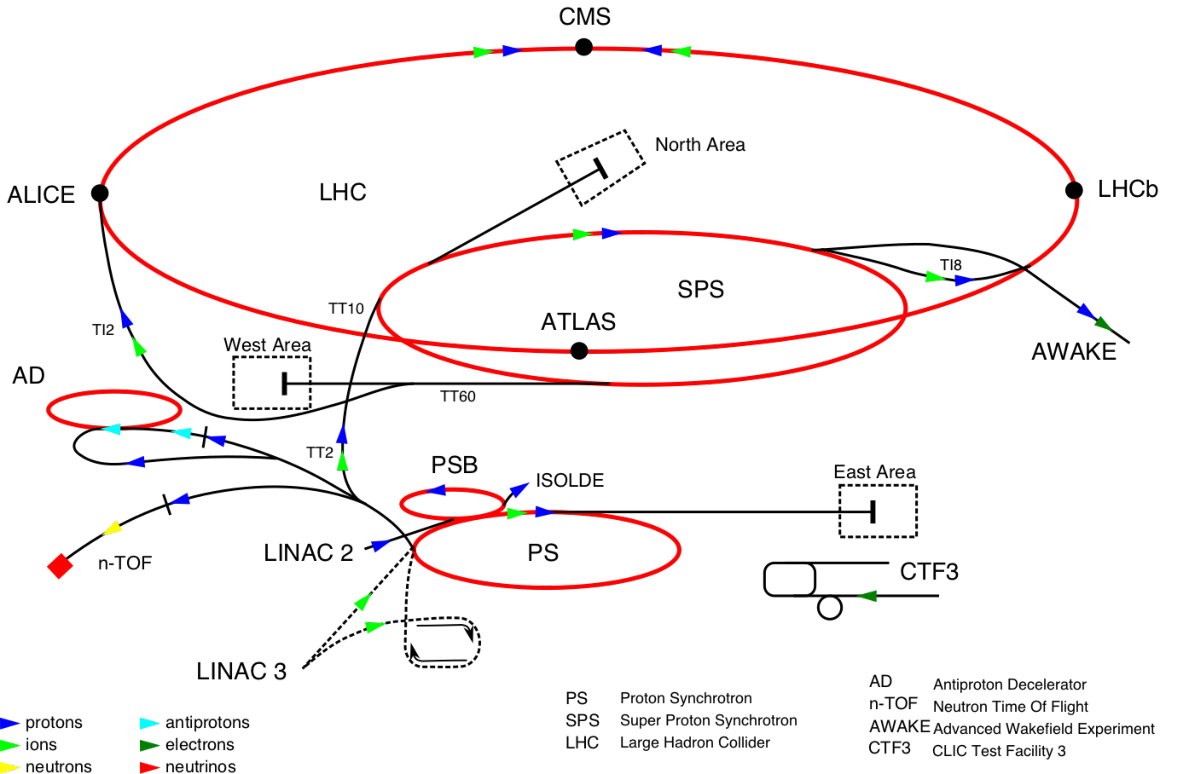
\includegraphics[width=0.9\textwidth]{figures/cerncomplex}
  \caption[Overview of the LHC accelerator complex]{Overview of the LHC accelerator complex~\cite{cerncomplex}.}
  \label{fig:cerncomplex}
\end{figure}
\begin{figure}[tb]
  \centering
  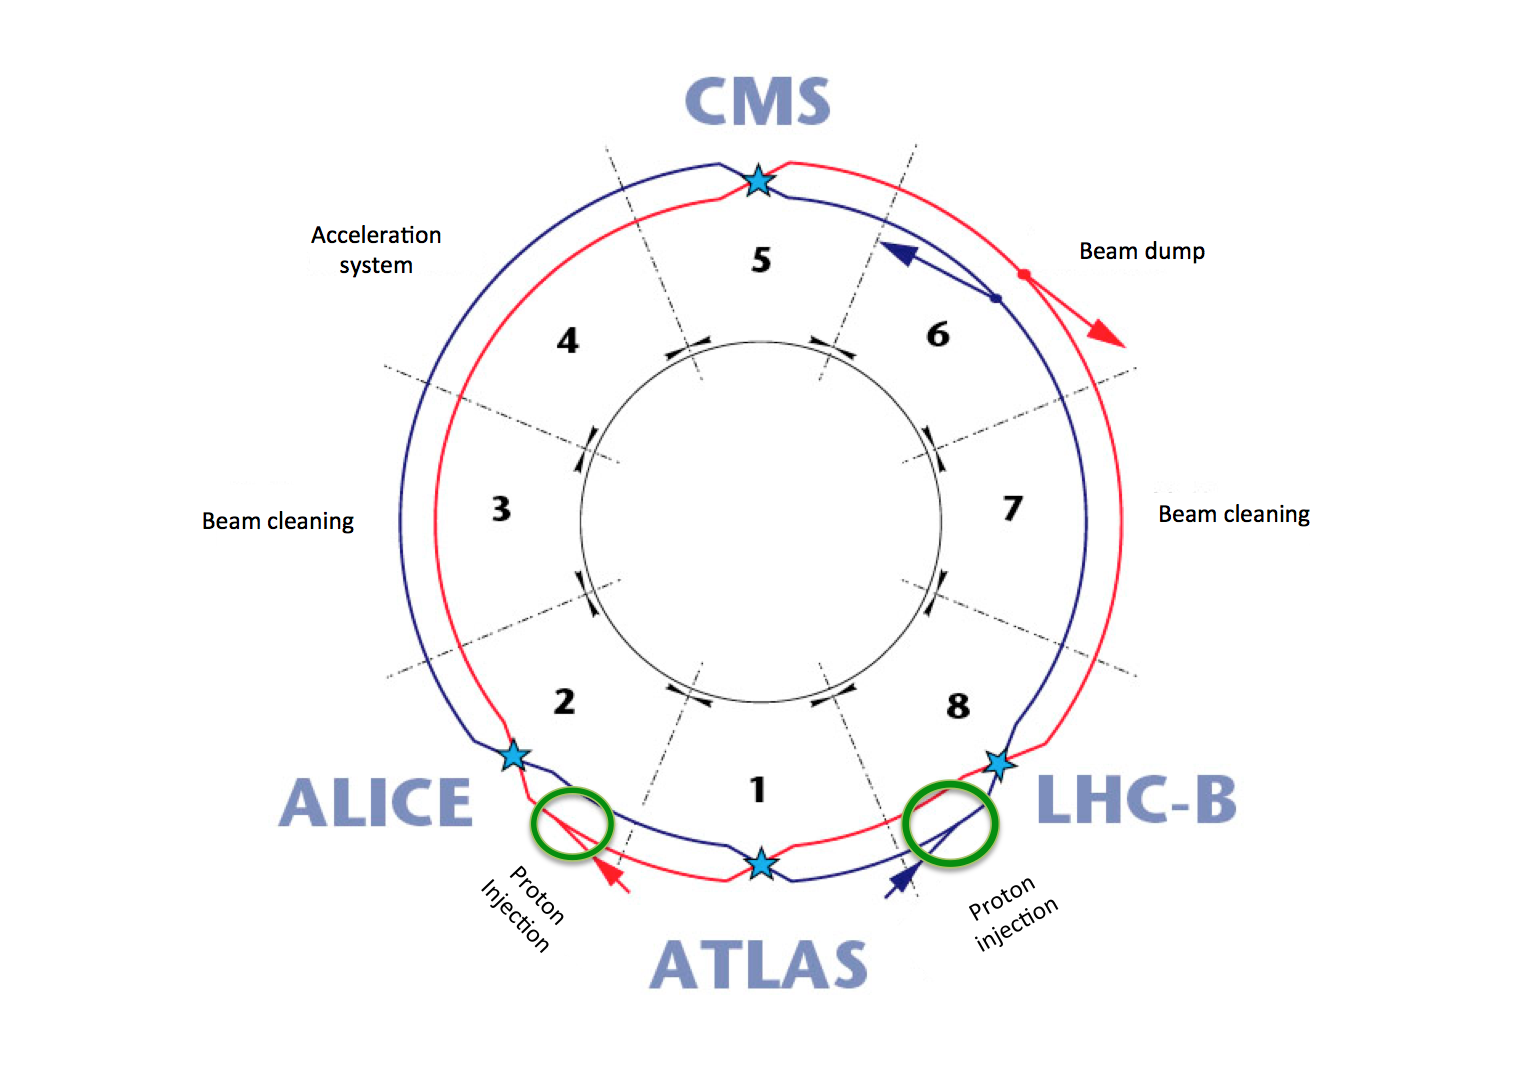
\includegraphics[width=\textwidth]{figures/lhc_schematic}
  \caption[Schematic layout of the LHC sectors]{Schematic layout of the LHC sectors~\cite{lhc_schematic}.}
  \label{fig:lhc_schematic}
\end{figure}
The following description of the LHC is based on~\cite{bluebook}. The LHC was
completed in 2008, at a cost of about \$4 billion (2008 USD), by the European
Organization for Nuclear Research, which is known by the acronym CERN (based on
its original name, Conseil Européen pour la Recherche Nucléaire).

An overview of the CERN accelerator complex is provided
in~\cref{fig:lhc_schematic}. The LHC was constructed in a \SI{26.7}{\km} tunnel
used in the 1980s for the Large Electron Positron (LEP) experiment. This tunnel
is roughly circular, composed of eight arcs and eight straight sections between
\SIrange{45}{170}{\meter} below ground level. The particle beams intersect at
four interaction points (IPs) located in four of the straight sections. The
protons are maintained in their trajectory around the ring via \num{1232} dipole
magnets, each \SI{14.3}{\meter} long with a field strength of \SI{8.3}{\tesla}.
The superconducting windings are copper-clad niobium-titanium and carry a
current of \SI{10980}{\ampere}~\cite{Willering:2017hrw}. There are also
\num{392} quadrupole magnets (between \SIrange{5}{7}{\meter}) that focus the
beam and keep it stable, while \num{6400} smaller magnets perform higher-order
corrections. The total energy stored in all of the magnets is about
\SI{10}{\giga\joule}. The magnets are cooled with \SI{96}{\tonne} of helium II,
which is helium at a temperature and pressure such that it displays superfluid
properties, namely zero viscosity. The low temperature, only~\SI{1.9}{\kelvin},
allows the conductors to remain superconducting at higher current densities and
magnetic fields than would be possible with helium I, and the superfluid state
of helium II allows it to remove heat about \num{10} times as
efficiently~\cite{Lebrun:1974065}.

LEP was a particle-antiparticle (electron-positron) collider, in which the
particles move in opposite directions but also had opposite charge;
consequently, both beams could share the same ring of magnets. The LHC is a
particle-particle (proton-proton) collider, however, and it requires two closely
spaced rings with opposite magnetic dipole fields. A twin-bore design was
adopted for the magnets to allow the two rings to fit within the existing
\SI{3.7}{\meter} diameter tunnel.

Protons are injected into the LHC using a series of accelerators recycled from
previous CERN experiments. The proton beam begins as hydrogen gas, which is
ionized by passing it through a charged screen and then accelerated to
\SI{50}{\mega eV} in the LINAC2 linear accelerator. The protons then enter the
Proton Synchotron Booster (PSB), a set of four rings of \SI{25}{\meter} radius
where they are accelerated to \SI{1.4}{\giga eV} and grouped into bunches. The
four beams from the PSB are merged and enter the \SI{100}{\meter}-radius Proton
Synchotron (PS). The PS was CERN's first synchotron, brought online in 1959. The
PS accelerates the protons to an energy of \SI{25}{GeV} before they are injected
into the Super Proton Synchotron (SPS)\footnote{The SPS began operation in 1979,
and the discovery of the W and Z bosons and CP violation were all made there.}.
The SPS has a radius of over a kilometer and accelerates protons to
\SI{450}{\giga eV}. Protons are diverted from the SPS into two separate
\SI{2.5}{\km} transfer tunnels that inject protons from opposite directions into
the clockwise and counterclockwise rings of the LHC. When both beams are filled,
the injection stops and the beams are pumped up to their peak energy. A beam
\textit{squeeze} is then performed in which the beams are focused, and finally,
the beam paths are brought together at the IP and collisions begin.

Running at \SI{6.5}{TeV} per proton with an intensity of \num{2.5e14} protons
per beam, the total energy\footnote{This is approximately equivalent to the
kinetic energy of 750 Honda Civics each moving at \SI{55}{MPH}, or the energy in
\num{319} chocolate bars.} in the beam is about \SI{260}{MJ}. The destructive
power of the beam necessitates a beam dump system\footnote{Some researchers have
proposed using the beam dump system itself to do physics such as dark matter
searches by placing a detector near the beam dump; see for
example~\cite{Kumar:2016qfv}.}. This system safely deposits this energy in the
case of any of a wide range of possible failures in the LHC (such as a magnet
\textit{quench} in which a magnet becomes non-superconducting) or at the end of
a physics run, after the luminosity of the beam has degraded below usable
levels. Each of the two LHC beams has a dump system that includes a set of fast
kicker magnets to deflect the beam and a septum magnet where the beam dump
channel branches from the circulating channel. The dumped beam is then directed
into an \SI{8}{\meter}-long cylinder of graphite composite that is encased in
concrete. A dilution magnet spreads the beam to minimize overheating; even under
normal operation, parts of the graphite can reach \SI{700}{\celsius}.
%260 MJ/(0.5 * (1,143 kg)(55 miles/h)^2) = 752.6

Protons circulating in the LHC are divided into a train of regularly spaced
bunches, each containing $\mathcal{O}(10^{11})$ protons. The particles are
accelerated as they pass through RF cavities; an electric field is induced
inside each cavity, which oscillates with a frequency that is an integer
multiple of the particle revolution frequency and is timed to apply an
accelerating force on each bunch of particles. During ramp up, as particles
travel around the ring, they receive an energy kick each time they pass through
a resonator, until they reach the target energy. At the LHC, the RF cavities
operate at \SI{400}{\mega\hertz} which corresponds to a ratio\footnote{The
protons are moving at approximately $c$, and the LHC has a circumference of
\SI{26659}{\meter}, so $f_\text{RF}/f_\text{rev} \approx \num{400e6} / (c /
\SI{26659}{\meter})=\num{35570}$.} between the RF and particle revolution
frequencies of \num{35570}. This value is the number of points, or
\textit{buckets}, circulating around each beam line, each of which can carry a
bunch of particles.

Not all the buckets contain bunches, however. The kicker magnets of the beam
dump system require \SI{3}{\micro\second} to reach full strength, and a
partially diverted beam would damage sensitive downstream accelerator
components. Consequently the beam contains a \SI{3}{\micro\second} \textit{abort
gap} of unfilled buckets; in the event of an abort the kicker magnets are
initiated at the start of the abort gap and reach full strength before the next
bunch of protons arrives.

The LHC was first brought online in 2008. Soon afterward, an electrical arc
damaged the cooling system, which resulted in a large helium
leak~\cite{2008LHCincident}. Over \num{50} magnets and additional components of
the cryogenic system were damaged. Initial operation was delayed by a year for
repairs as well as to carry out a detailed investigation and implement
preventative measures. In 2010 the LHC began operations at a record-breaking
center-of-mass energy ($\sqrt{s}$) of~\SI{7}{TeV}, exceeding the previous record
of $\sqrt{s}=\SI{1.96}{TeV}$ set by the Tevatron, which ceased operations in
2011. In April 2012 the beam energy was increased to 8 TeV and remained at that
level for the duration of 2012. This period is referred to as Run 1. After Run
1, the LHC began the first ``long shutdown" (LS1) to make necessary upgrades for
raising the center-of-mass energy. In June 2015, physics data collection resumed
at $\sqrt{s}=\SI{13}{TeV}$. This point was the beginning of the data-taking
period referred to as Run 2, which is scheduled to conclude in 2018. This thesis
presents analyses based on both datasets.

Charged particles undergoing acceleration emit bremsstrahlung radiation. For
circular motion, the radiated power due to centripetal acceleration is
proportional to $\SI{}{1\per\m^4}$. A significant advantage of proton-proton
colliders over electron-positron colliders like LEP is the fact that, because of
the higher proton mass, less energy is lost to bremsstrahlung radiation.
However, in contrast to an electron-positron collider like LEP, where all of the
energy in a collision is available to produce final state particles, the
momentum in a proton is divided between its constituent partons. The momentum
carried by a given parton follows a statistical distribution. So while less
energy is lost to bremsstrahlung radiation in a proton-proton collider, allowing
it to produce higher energy projectiles, only some collisions are produced near
the proton-proton center-of-mass energy provided by the accelerator.

In a search for rare events, a critical metric is the rate at which the
interaction of interest occurs. This rate is proportional to the luminosity,
which provides a measure of the rate at which particles pass through the
interaction volume, and the cross section, which is the probability that each
particle will experience the interaction of interest. The dimensions of
luminosity are \SI{}{(area)^{-2}\second^{-1}}. If Gaussian beams collide
head-on, the instantaneous luminosity is~\cite{Herr:941318}:
\begin{equation}
  \mathcal{L} = \frac{N_b^2 n_b f \gamma}{4 \pi \sigma_{xy}}
  \label{luminosity}
\end{equation}
where $N_b$ is the number of particles per bunch, $n_b$ is the number of bunches
per beam, $f$ is the revolution frequency, $\gamma$ is the relativistic gamma
factor, and $\sigma_{xy}$ is the transverse beam size.

Real machines such as the LHC have additional complications. Collisions are not
head-on, but occur at a small but non-zero crossing angle. This circumstance
introduces a factor $S$ in the luminosity equation, which for small crossing
angles and bunch length $\sigma_z \gg \sigma_{xy}$ is approximated as
\begin{equation}
  S = \frac{1}{\sqrt{1 + (\frac{\theta_z}{\theta_x} \frac{\phi}{2})^2}}.
\end{equation}

Additionally~\cref{luminosity} assumes that the entire collision region has a
constant beam size. In fact the transverse beam size is a function of the
distance along the beam trajectory. To maximize the number of expected
collisions, the focusing fields are designed to minimize beam size at the IP.
The beams spread out in both directions, creating an hourglass shape that is
characterized by the amplitude function $\beta(z)$ and the beam emittance
$\epsilon$, where
\begin{equation}
  \theta_{xy}(z) = \sqrt{\epsilon \cdot \beta(z)}.
\end{equation}

An important metric describing the extent to which the beam is ``squeezed" is
the $\beta^*$ value, which gives the distance from the IP at which the
transverse beam size doubles. For Runs 1 and 2, $\beta^*$ was typically
\SIrange{40}{60}{\centi\meter}.

Although multiple proton-proton collisions (\textit{events}) occur per crossing,
there are far fewer interesting high-$p_T$ scattering events. The majority of
the collisions simply produce sprays of hadrons along the beamline that
complicate reconstruction of interesting events. The occurrence of multiple
collisions per bunch crossing is referred to as \textit{pileup}; mitigating the
effects of pileup by filtering out particles from uninteresting collisions
during the reconstruction process is essential to the detection of rare events.

In both runs, the number of protons per bunch is $\mathcal{O}(10^{11})$. In Run
1, beam stability issues limited the number of bunches per beam to \num{1380}
with a bunch crossing every \SI{50}{\nano\second} and an average of 21
proton-proton collisions per bunch crossing.  During Run 2, most of the data
were obtained with a bunch crossing every \SI{25}{\nano\second} and an average
of \num{27} collisions per bunch crossing. The maximum instantaneous luminosity
reached during Run 1 was~\SI{7.7}{\hertz\per\nano b}. In total, about
\SI{30}{fb^{-1}} of proton-proton data were delivered during Run 1. Integrated
and instantaneous luminosity along with pileup are presented
in~\cref{fig:luminosity} for 2012 (representative of Run 1) versus 2016
(representative of Run 2).

\begin{figure}[!htb]
  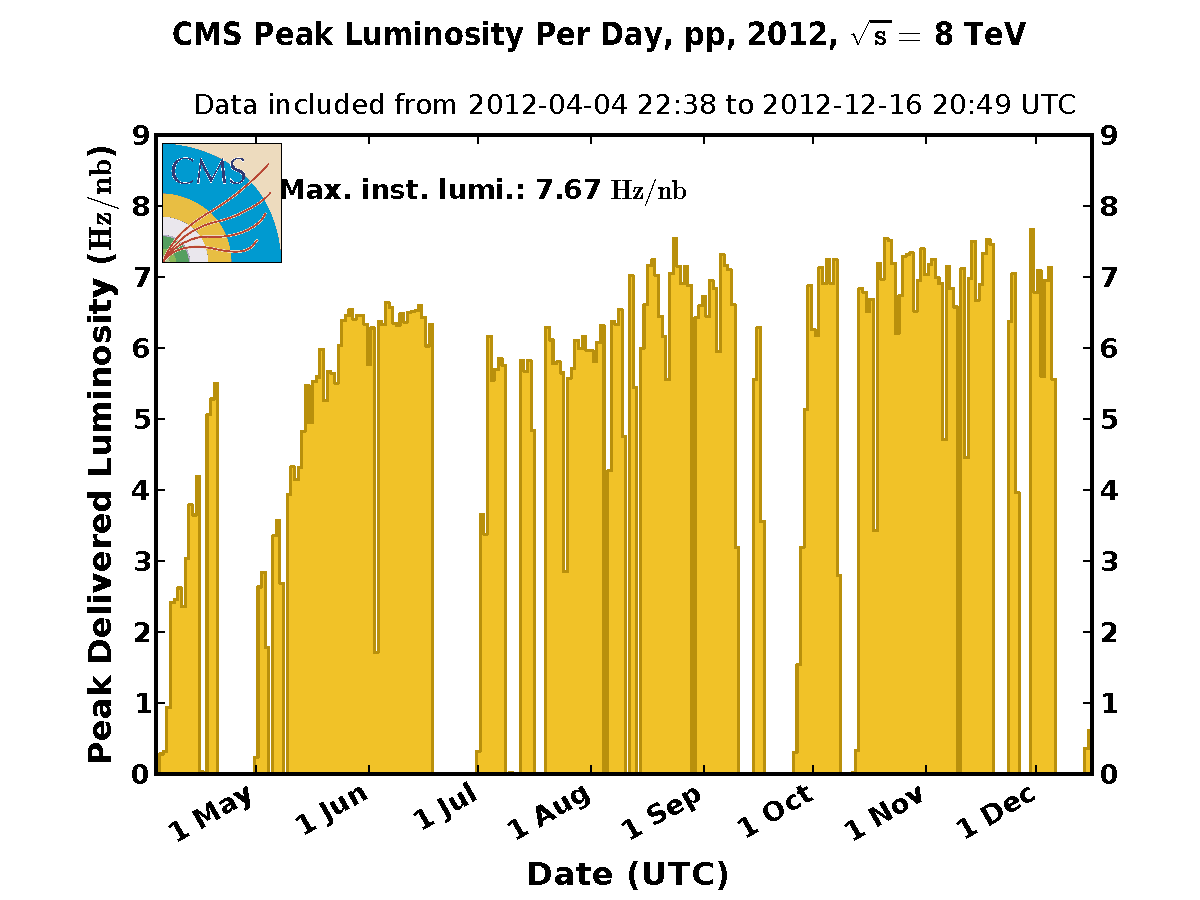
\includegraphics[width=0.49\textwidth]{figures/peak_lumi_per_day_pp_2012}
  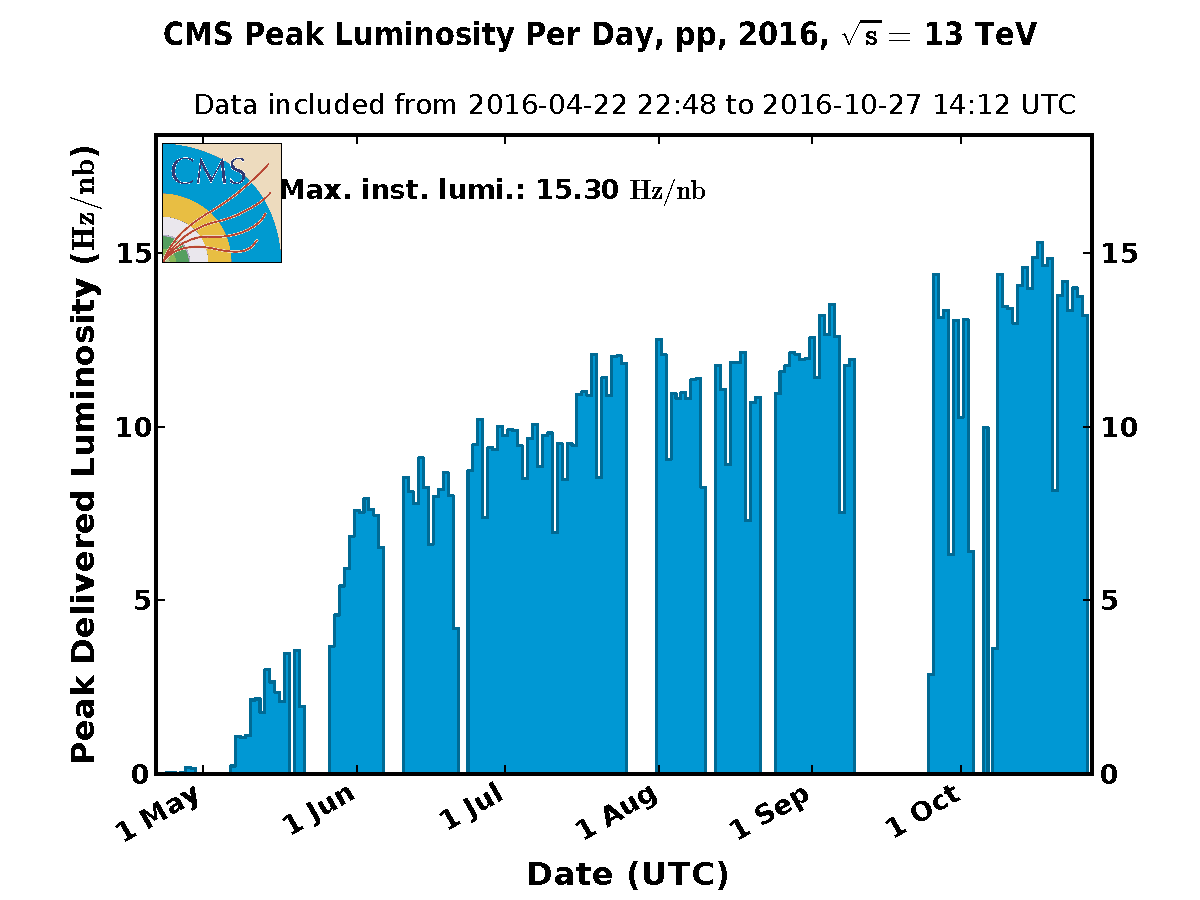
\includegraphics[width=0.49\textwidth]{figures/peak_lumi_per_day_pp_2016}
  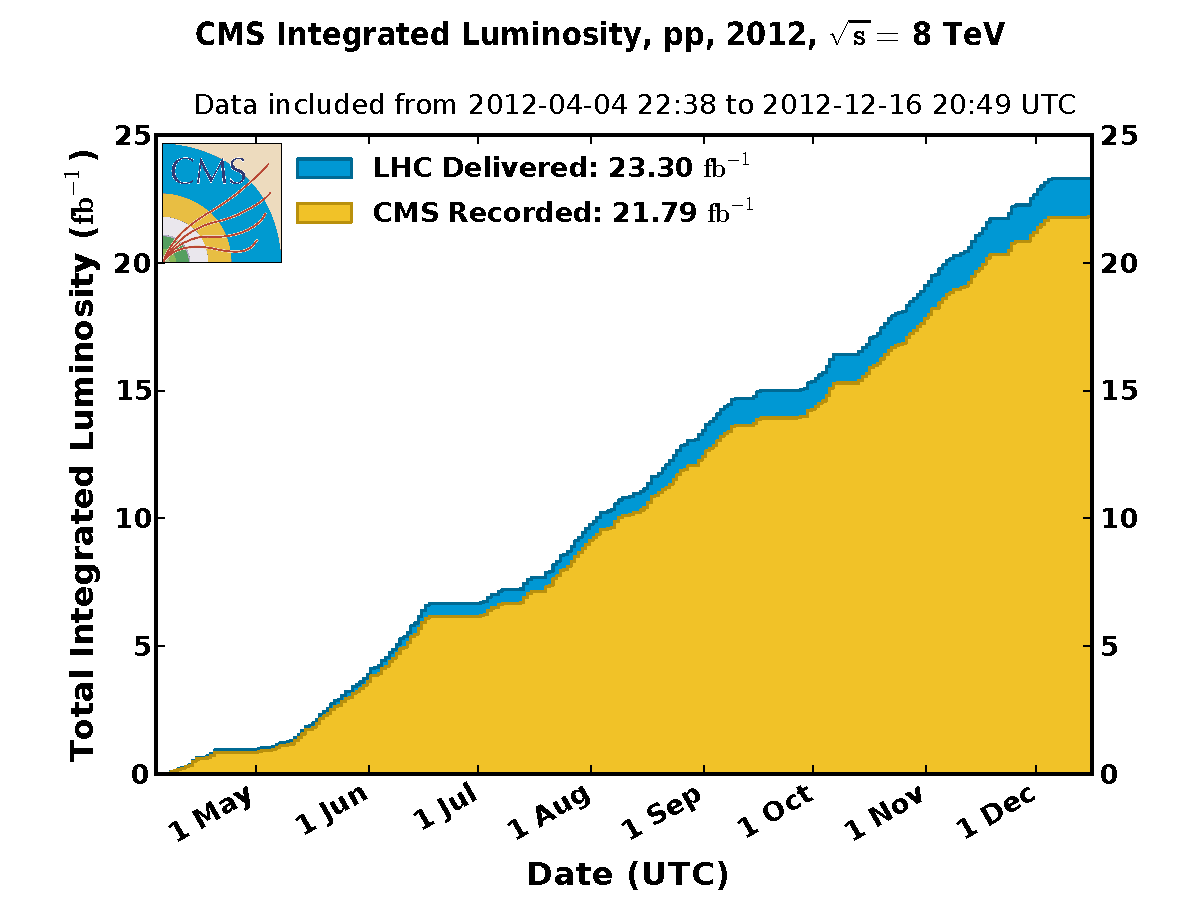
\includegraphics[width=0.49\textwidth]{figures/int_lumi_per_day_cumulative_pp_2012}
  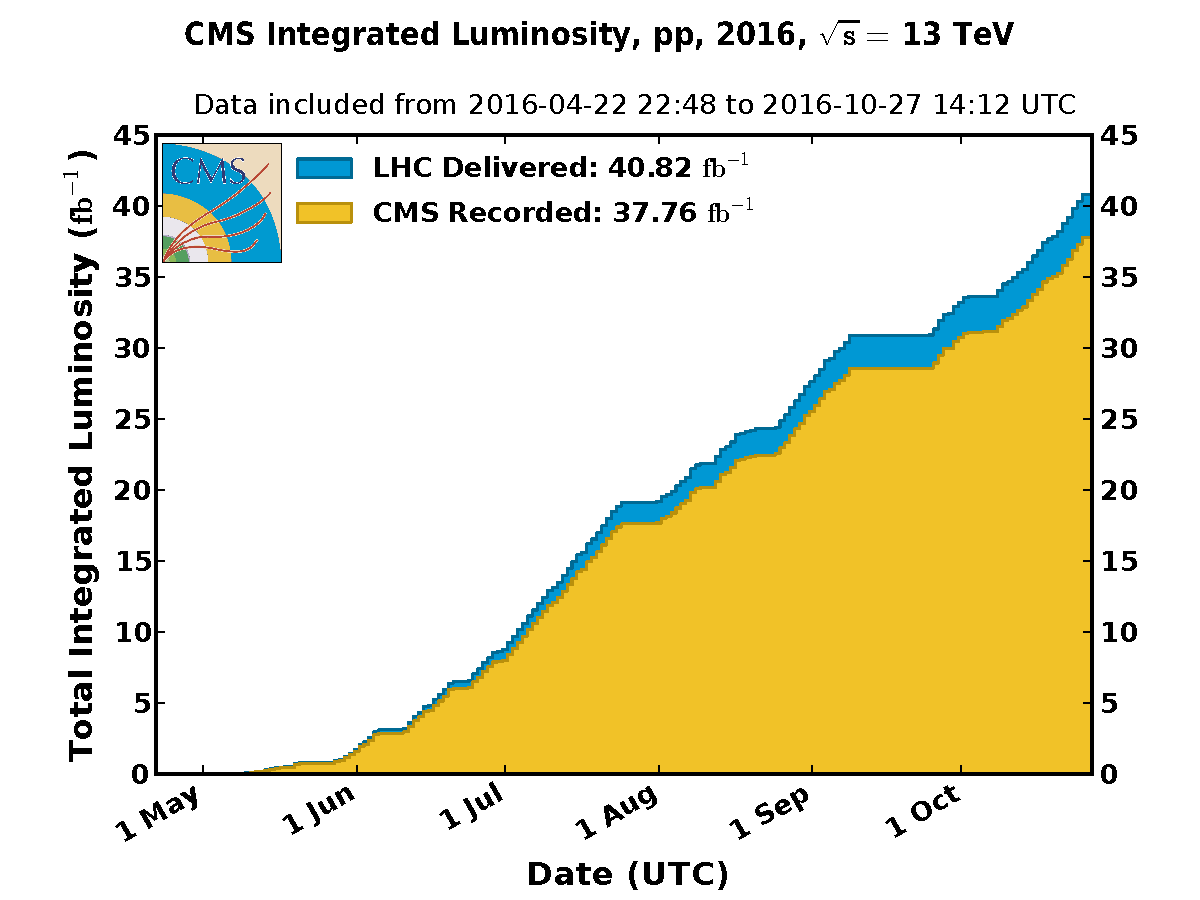
\includegraphics[width=0.49\textwidth]{figures/int_lumi_per_day_cumulative_pp_2016}
  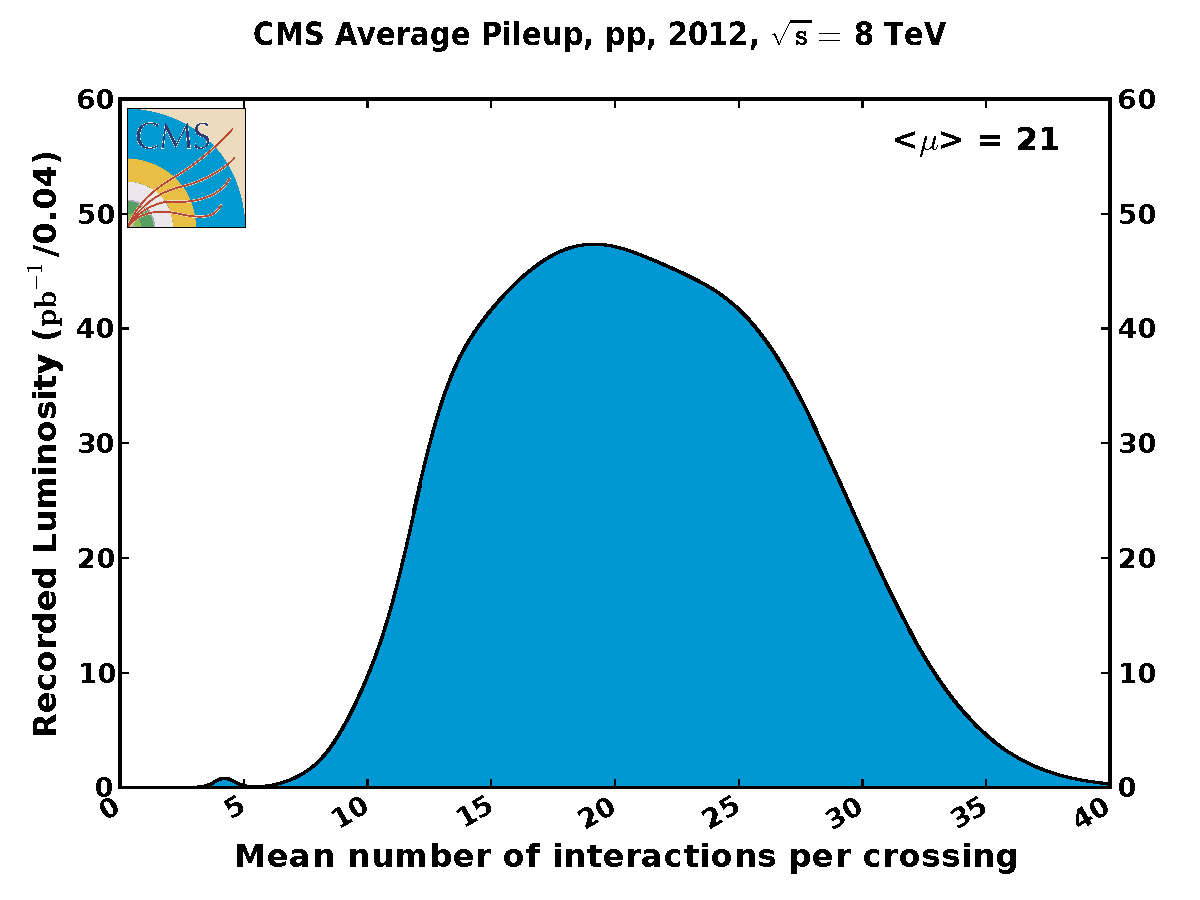
\includegraphics[width=0.49\textwidth]{figures/pileup_pp_2012}
  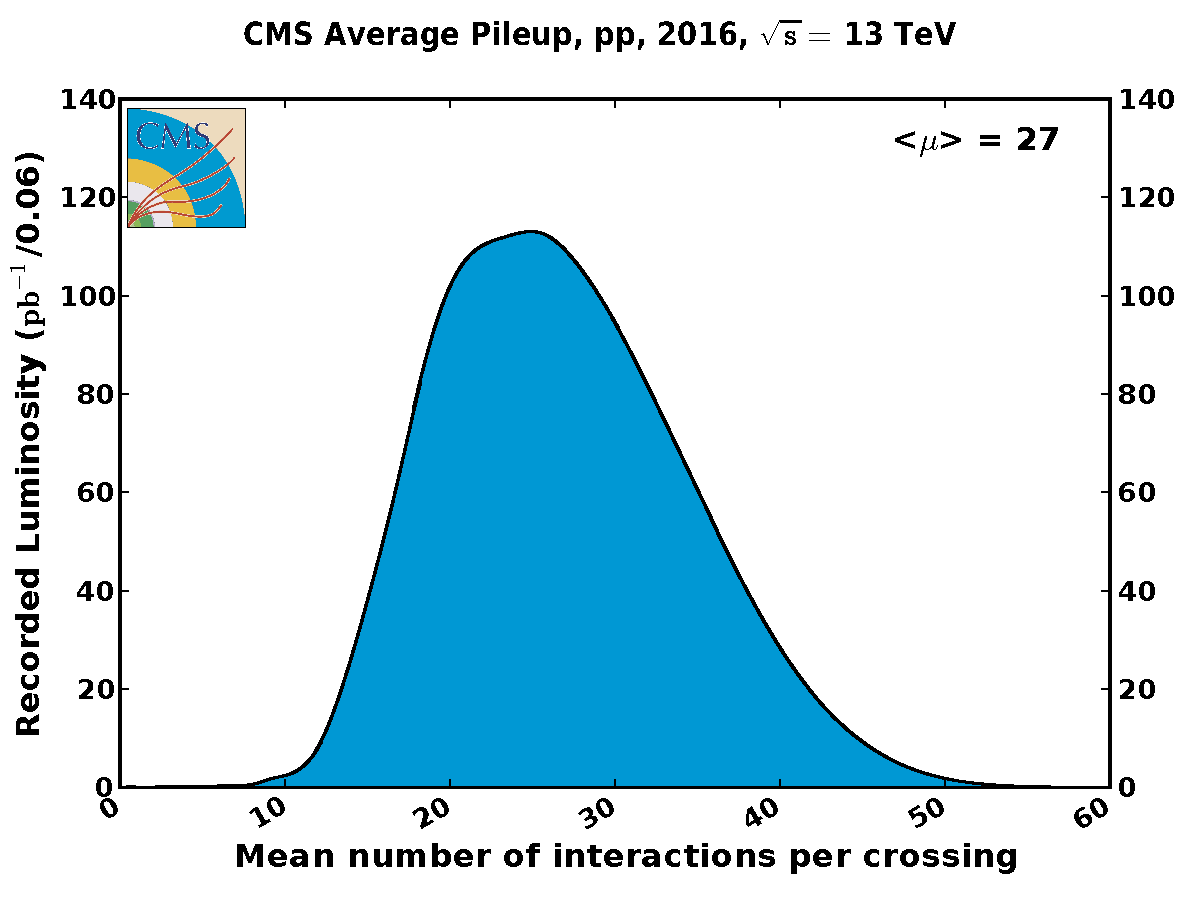
\includegraphics[width=0.49\textwidth]{figures/pileup_pp_2016}
  \caption[Luminosity and average pileup at CMS]{
  Maximum instantaneous luminosity (top), integrated luminosity (center), and
  mean interactions per crossing (bottom) at CMS for 2012 (left) and 2016
  (right)~\cite{cmslumi}.
  }
  \label{fig:luminosity}
\end{figure}

\section{The CMS detector}
\label{sec:cms}

\subsection{Overview}
\label{sec:cms-overview}
CMS (see~\cref{fig:cms-overview} and~\cref{fig:cms-slice}) is located at IP 5
near the French town of Cessy, in a cavern about \SI{100}{\meter} underground.
The name Compact Muon Solenoid reflects the special attention given to muon
detection and the solenoid coil that surrounds the detector elements with a
strong magnetic field. It is roughly cylindrical, measuring about
\SI{21.6}{\meter} in length and \SI{15}{\meter} in diameter and weighing about
\SI{14000}{\tonne}. CMS is less than half the length of ATLAS and a little over
half its diameter, while being significantly more massive. This status may be
the source of the term ``compact"~\footnote{Both detectors are ``compact'' in
comparison to other larger detectors, like the Laser Interferometer
Gravitational Wave Observatory, which has two observatories each with
\SI{4}{\kilo\meter} interferometer arms.}. The CMS collaboration consists of
approximately \num{3800} people at about \num{199} institutions in \num{43}
countries. The total cost for design and construction of the CMS was about \$510
million (2008 USD).
\begin{figure}[tb]
  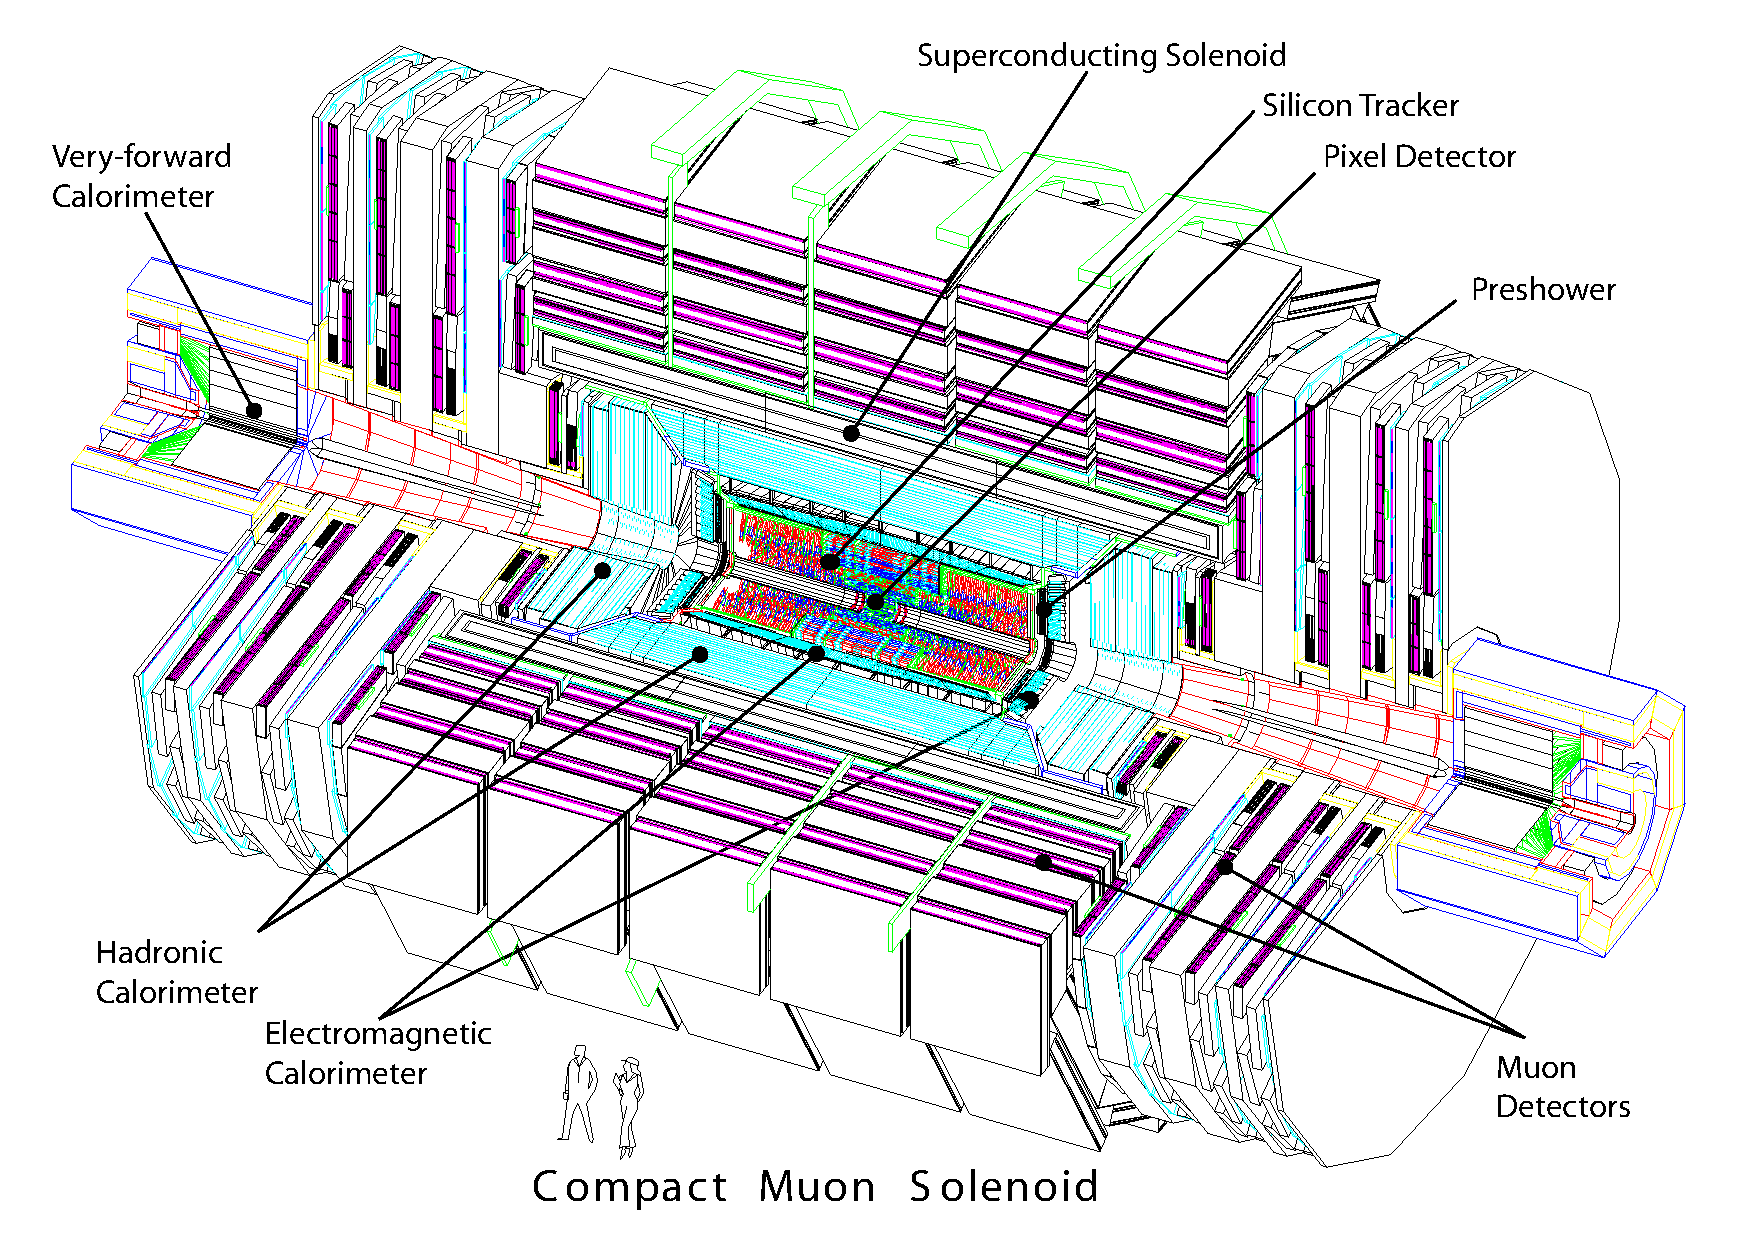
\includegraphics[width=0.7\textheight]{figures/cms_complete_labelled}
  \caption[Overview of the CMS detector]{Overview of the CMS
  detector and its subcomponents~\cite{cms-tdr-1}.}
  \label{fig:cms-overview}
\end{figure}
\begin{figure}[tb]
  \centering
  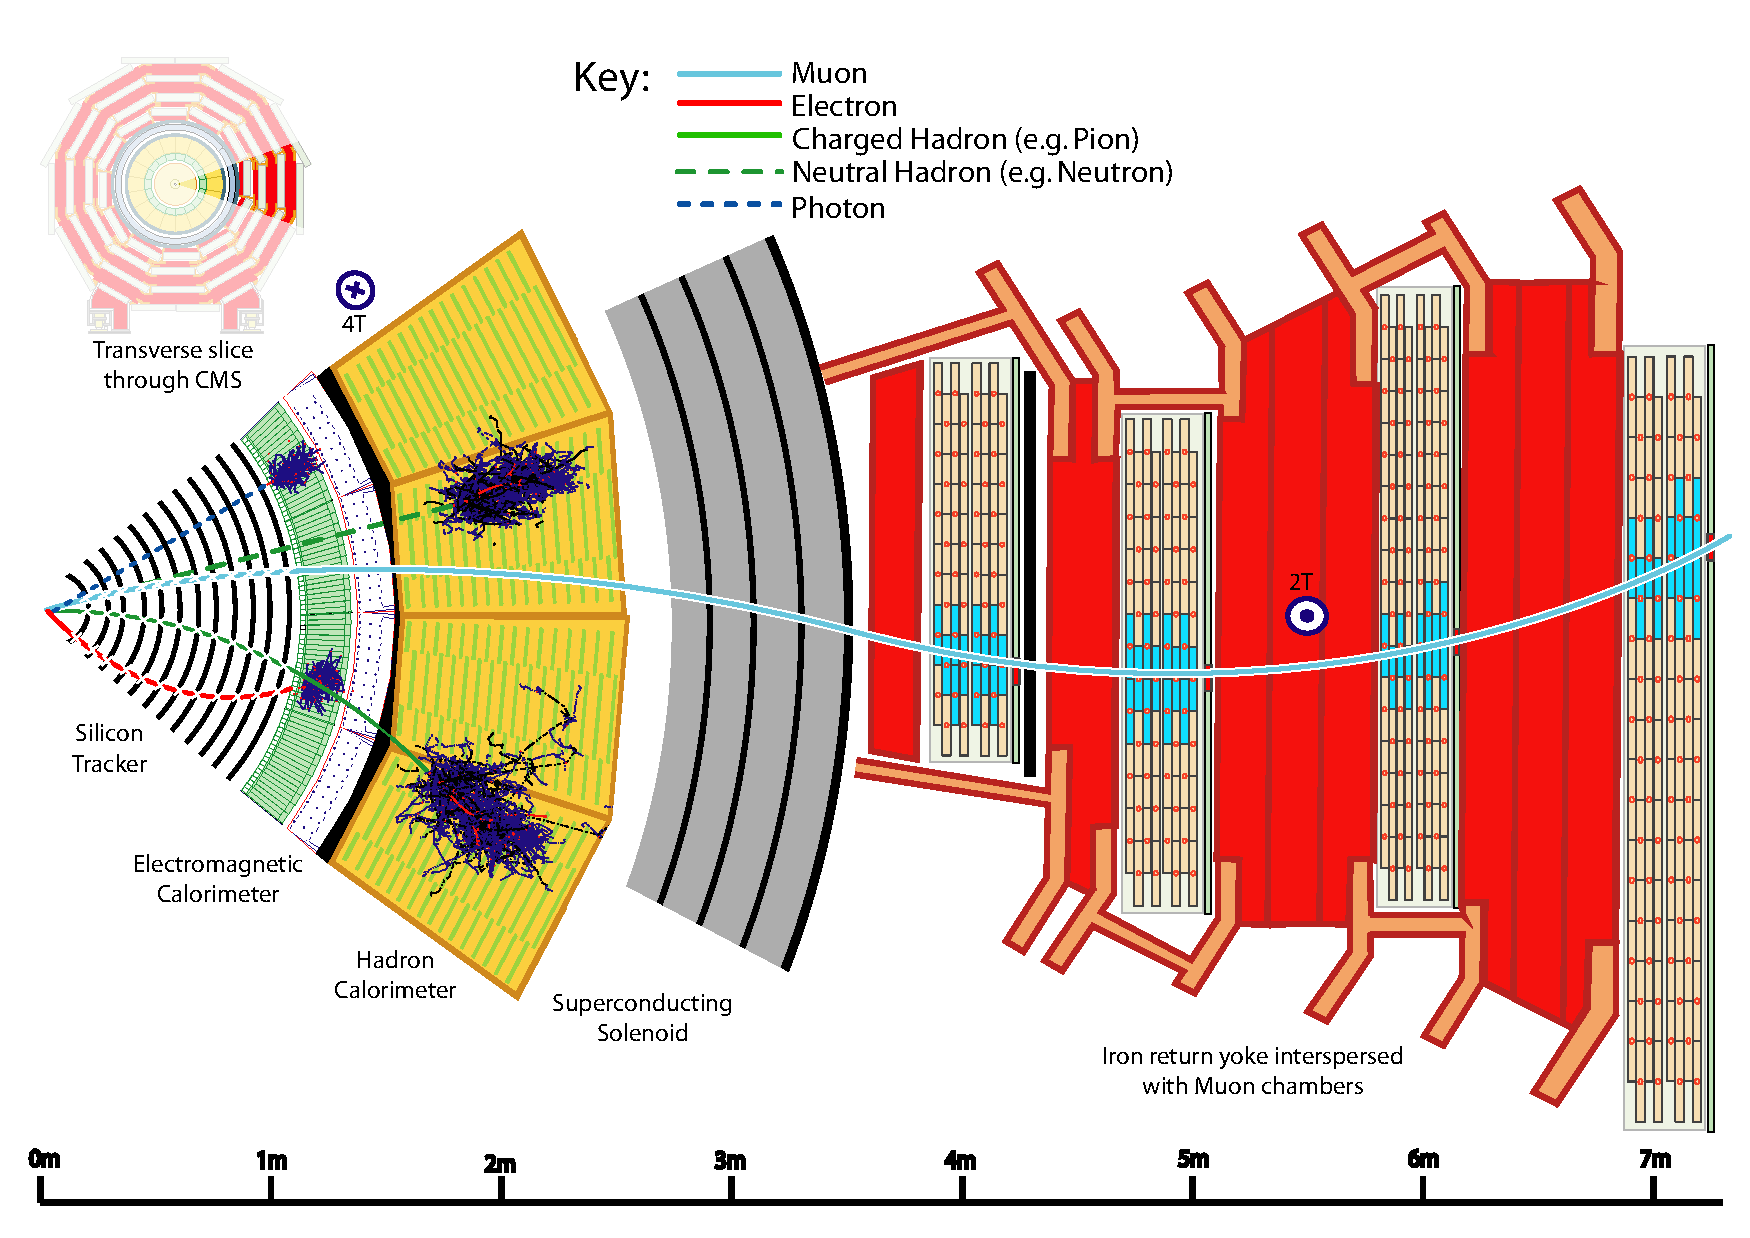
\includegraphics[width=0.7\linewidth]{figures/cms_slice_white}
  \caption[Transverse slice through the CMS detector]{Transverse slice
    through the CMS detector.  Particle traces are depicted to
  illustrate the function of the components~\cite{cmsoutreach}.}
  \label{fig:cms-slice}
\end{figure}

CMS is a general-purpose detector, designed to characterize a wide range of
proton-proton scattering events. Consequently, the design had to be hermetic, in
order to record the energy, charge, and momentum of as many scattering products
as possible. The detector is made up of a cylindrical barrel and two endcaps
with its longitudinal axis along the beamline.

Events produce a variety of final state particles that participate in different
sets of fundamental interactions. For this reason, CMS is composed of multiple
subdetectors, each optimized for measurements of specific sets of particles. A
central feature of CMS is its solenoid magnet, which produces a strong and
roughly constant magnetic field around the IP. Charged particles moving in a
magnetic field will follow a curved path with a radius that is proportional to
the momentum. A \textit{tracker} detects the ionization left by the passage of a
charged particle. If at least three points along the particle's path can be
determined, it is possible to reconstruct the radius of its trajectory and
calculate its momentum to charge ratio. Since leptons and stable hadrons have
integer units of elementary charge, particle momentum and the sign of its
assumed unit of charge (reflected in the sign of the track curvature) can be
reconstructed in practice.

A tracker alone is not sufficient to fully characterize events: neutral
particles will pass through undetected, and particles with different masses can
have the same momentum. To fully characterize a particle, only one unknown is
permitted in the equation $E^2 = p^2 + m^2$. For these reasons, CMS includes
\textit{calorimeters} that measure particle energy. Because the calorimeters
stop particles, the tracker must be the innermost detector; conversely, energy
loss in the tracker must be minimized to allow particle energy to be measured
accurately in the calorimeter.

Charged particles moving through matter are accelerated in the coulomb field of
atomic nuclei and emit bremsstrahlung radiation. Power loss for muons is
suppressed compared with electrons because of their higher mass, and as a
result, muons are not easily stopped in the calorimeters. A dedicated muon
tracking system is placed outside the calorimeters. Because other particles are
stopped in the calorimeters, a sign-of-charge (sign of track curvature) and
momentum measurement (radius of track curvature) are sufficient to fully specify
muons. One final type of particle, the neutrino, only interacts weakly and thus
is invisible to both trackers and calorimeters. By making the detector as
hermetic as possible, the presence of neutrinos or exotic neutral particles can
be inferred using conservation of momentum (see~\cref{sec:coordinates}).

The following sections describe the CMS components in more detail and are based
on~\cite{1748-0221-3-08-S08004}.

\subsection{Coordinate system and conventions}
\label{sec:coordinates}
The standard CMS coordinate system is used throughout this work, in which the
origin is defined as the nominal interaction point. The x-axis points towards
the center of the LHC ring, the y-axis points upwards towards the sky, and the
z-axis points along the beamline such that the system is right-handed.
Alternatively, polar coordinates are defined such that the distance from the
beamline in the plane perpendicular to the z-axis is called $r$. The azimuthal
angle $\phi$ is defined such that $\phi=0$ points along the x-axis. The polar
angle is defined such that $\theta=0$ points along the z-axis.

Conservation of momentum requires that the total outgoing particle momenta
equals the total incoming parton momenta. Because the momentum vector of the
incoming protons is entirely along the beamline, the momentum in the plane
transverse to the beamline must sum to zero, while the longitudinal component
depends on the unknown fraction of the total proton momentum that each parton
carried. Thus, longitudinal boosts vary from event to event in a distribution
that depends on the parton distribution functions (PDFs). For this reason, we
are usually only concerned with the transverse component of momentum \pT, from
which the transverse energy $E_T$ is defined for a particle of mass $m$:
\begin{align}
  \pT &= |\vec{p}| \sin\left(\theta\right) = \sqrt{p_x^2 + p_y^2}, \\
  E_T &= \sqrt{m^2 + \pT^2}.
\end{align}
Any deviation of the total transverse momentum from zero must have been carried
away by weakly interacting particles such as neutrinos. This quantity is called
the \textit{missing transverse momentum}: $\pTmiss = \abs{- \sum_i
\vec{p}_{T,i}}$, where the sum is over $i$ visible particles.
\todo[inline]{spacing is messed up in math mode}

The rapidity $y$ and the pseudorapidity $\eta$ are defined in terms of $\theta$:
\begin{align}
  y &= \frac{1}{2}\ln\left(\frac{E+p_z}{E-p_z}\right) \\
  \eta &= \frac{1}{2}\ln\left(\frac{|\vec{p}|+p_z}{|\vec{p}|-p_z}\right) = -\ln\tan\frac{\theta}{2}.\label{eq:eta}
\end{align}
The rapidity has the desirable feature that differences in rapidity are
invariant under boosts along the beam axis. Characterizing angles between
outgoing particles in terms of such a quantity allows for more convenient
comparison of events with different boosts. In other words, a histogram showing
the rapidity separation between two particles is meaningful despite being
populated by events whose center-of-mass frames have arbitrary longitudinal
boosts. The rapidity depends on both energy and momentum, which is difficult to
measure at high rapidities for highly relativistic particles. For this reason,
it is more common to work with the pseudorapidity, which is approximately equal
to the rapidity in the limit $|\vec{p}| \gg m$ because $E^2 = \abs{\vec{p}}^2 +
m^2 \implies E \approx |\vec{p}|$. It follows from~\cref{eq:eta} that $\eta=0$
corresponds to the vector perpendicular to the beamline, and $\eta=\infty$
($\eta=-\infty$) corresponds to a vector that is parallel (anti-parallel) to the
beamline. As $\eta$ gets closer to the beamline, equally spaced angular
separations represent larger and larger changes in $\eta$. This reflects the
intuitive fact that due to events being randomly boosted in the forward
directions (along the beamline), the average flux of particles is much higher in
the forward directions (at angles close to the beamline).

The angular separation in $\operatorname{\phi-\eta}$ space that describes solid
angles is called $\Delta R$, and it is also approximately Lorentz invariant.
$\Delta R$ is defined as
\begin{equation}
  \Delta R = \sqrt{\Delta\eta^2 + \Delta\phi^2}.
\end{equation}

\subsection{Solenoidal magnet}
The CMS magnet is a solenoid \SI{6}{\meter} in diameter and \SI{12.5}{\meter} in
length, capable of producing a highly uniform magnetic field in its inner bore.
It is large enough to accommodate the tracker and calorimeters, in order to
minimize energy losses when traversing the magnet, which would interfere with
their measurements. The standard operating field of \SI{3.8}{\tesla} requires a
current of~\SI{18160}{\ampere}, corresponding to a stored energy of
\SI{2.3}{\giga\joule}, which circulates in four layers of superconducting
niobium-titanium windings. A \SI{10000}{\tonne} steel return yoke, composed of
five barrel wheels and six endcap disks, guides the lines of magnetic field
around the outside of the solenoid and back into the other end. The return yoke,
because of its ferromagnetism and high magnetic permeability, becomes magnetized
by the field and thus passively adds to the field strength, focusing the field
in the region outside the solenoid where the muon system is located.

Charged particles moving inside the solenoid are deflected by the Lorentz force,
$\vec{F} = q(\vec{v} \times \vec{B})$. This force causes the component of the
particle velocity that is perpendicular\footnote{At CMS, the magnetic field
points along the z axis, so the component perpendicular to it is the transverse
component described in~\cref{sec:coordinates}.} to the magnetic field $v_T$ to
produce circular motion while the component of velocity parallel to the magnetic
field is unaffected, which results in a helical trajectory. Particle momentum
and charge can be determined from the radius and direction of curvature of the
particle's trajectory.

The windings of the solenoid are superconducting, which requires the magnet to
be cooled with liquid helium. One component in the cryogenic system is the cold
box, which contains the liquid helium heat exchangers. Run 1 went mainly
smoothly for the CMS magnet. Unfortunately, the cold box became contaminated by
oil in some components early in Run 2, causing erratic performance. As a result
only about \SI{75}{\percent} of 2015 proton-proton collision data were taken at
full magnetic field strength. During the year-end technical stop the affected
components were thoroughly cleaned and the oil recovery system was upgraded.
Magnet operation has subsequently run smoothly.

\subsection{Inner tracker}
\begin{figure}[htb]
  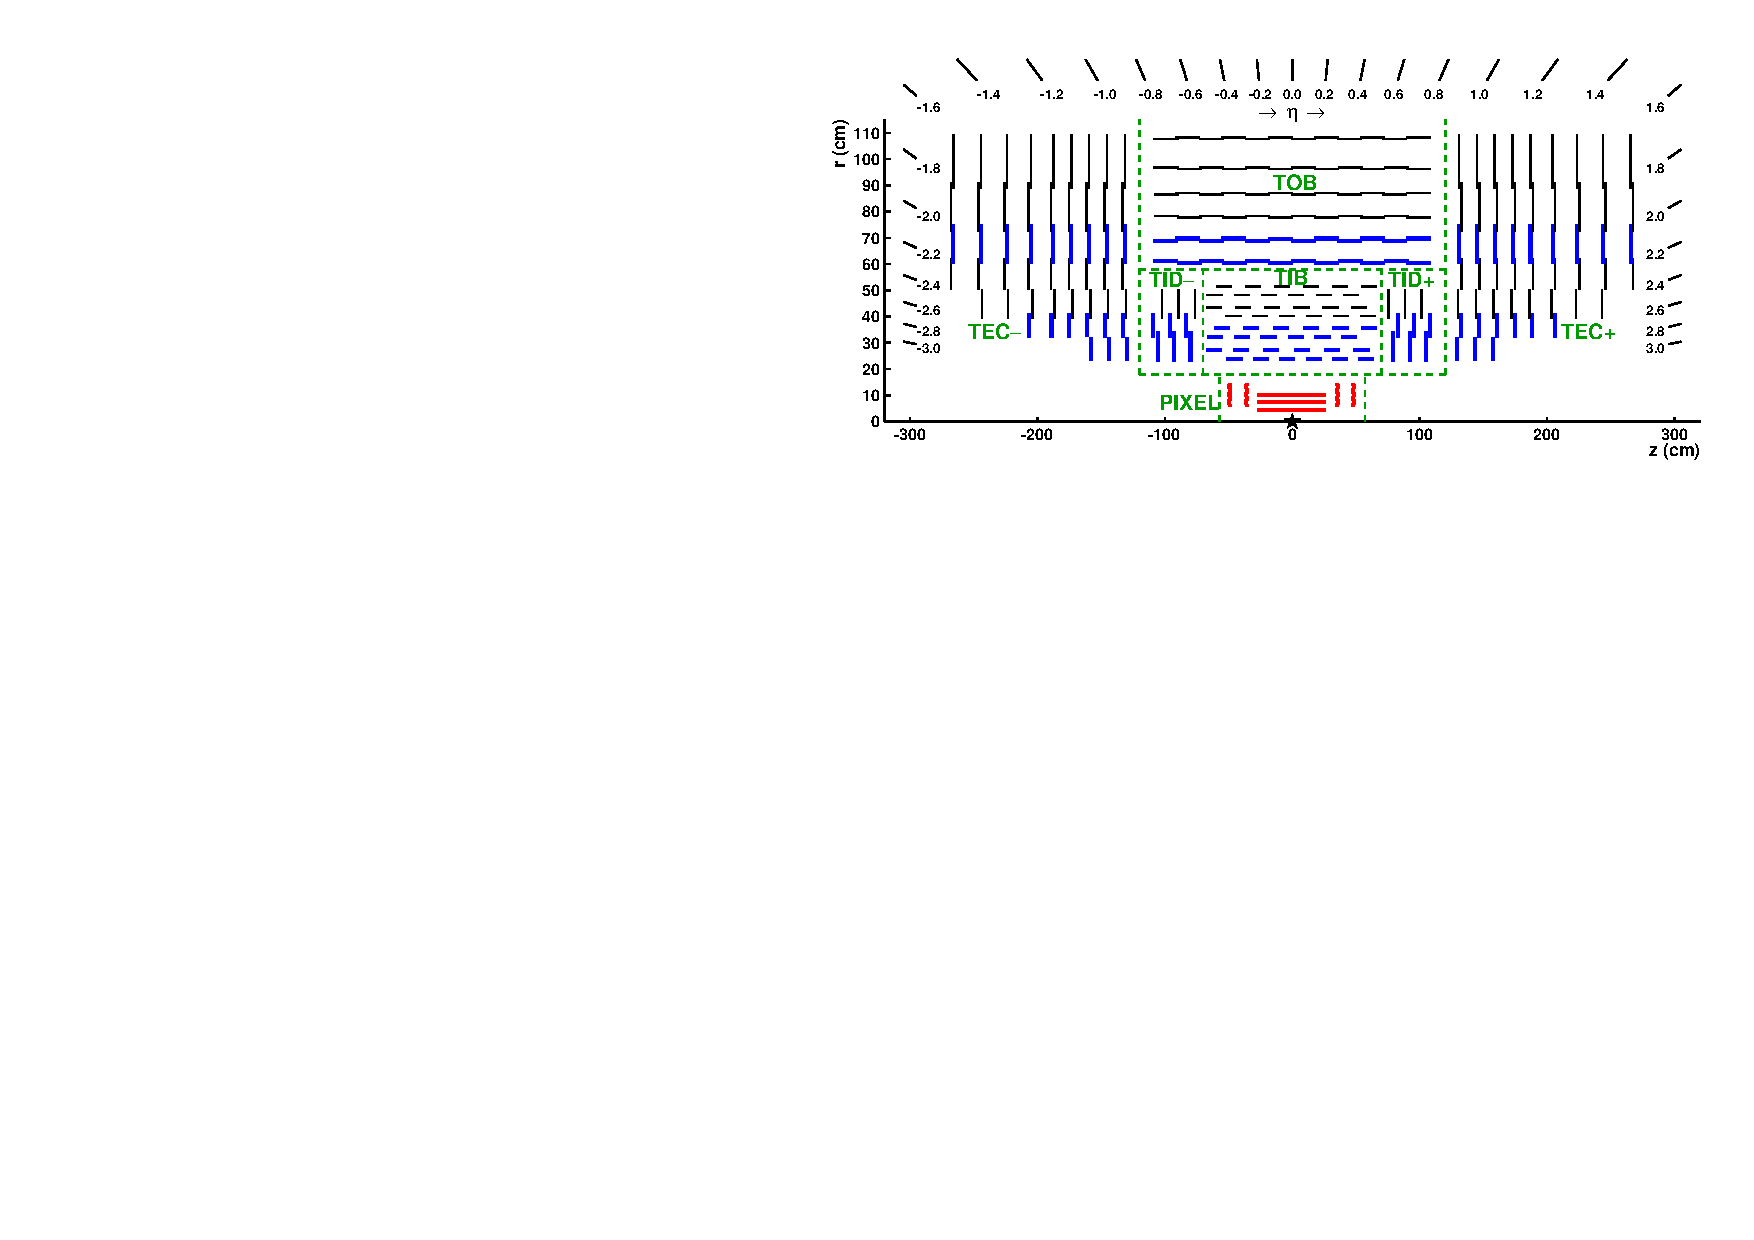
\includegraphics[width=\textwidth]{figures/tracker}
  \caption[Longitudinal cross section of the CMS inner tracker]{Longitudinal cross section of the CMS inner tracker~\cite{Chatrchyan:2014fea}.}
  \label{fig:tracker}
\end{figure}
The CMS inner tracker~\cite{tracker1,tracker2} (pictured in~\cref{fig:tracker})
is a cylindrical subdetector that is closest to the IP, consisting of an inner
silicon pixel detector and an outer silicon strip detector. It is designed to
measure the location and time that an electrically charged particle passes (a
\textit{hit}) while inducing minimal energy loss. Minimizing energy loss
requires the tracker to be capable of taking such accurate hit measurements that
the particle trajectory (or \textit{track}) can be reconstructed with just a few
hits. Being the innermost subdetector, it receives the highest flux of particles
and therefore radiation hardness is very important. The inner tracker covers
$|\eta|<2.5$ and has about \SI{200}{\meter^2} of active silicon area, which is
approximately the size of a tennis court. In the central region, the inner
tracker has a typical momentum resolution of \SI{0.7}{\percent} at \SI{1}{GeV}
and \SI{5.0}{\percent} at \SI{1000}{GeV}~\cite{Khachatryan:2010pw} and typical
impact-resolution for high momentum tracks of \SI{10}{\micro\meter}.
Unfortunately, the material making up the tracker corresponds to up to 0.5
interaction lengths at some pseudorapidities, which means that in the worst case
up to an \SI{85}{\percent} chance exists for a photon to convert or an electron
to emit bremsstrahlung radiation, and hadrons have a \SI{20}{\percent}
probability of a nuclear reaction before entering the
calorimeters~\cite{Sirunyan:2017ulk}. These interactions complicate event
reconstruction.

Silicon detectors are semiconductors, with electrical properties that are
determined by introducing small amounts of impurities that add mobile charge
carriers. N-type silicon has electron charge carriers, while p-type silicon has
lattice positions from which an electron is missing, resulting in mobile
\emph{holes}. The detector contains a junction between n-type and p-type
regions. An externally applied voltage provides a positive charge to the n-type
region, drawing electrons away from the junction, while a negative charge
applied to the p-type region draws away holes. This produces a region with no
mobile charge carriers near the junction, called the depletion zone, and no
current flows. The detector is a diode under reverse bias.

When a charged particle passes through the detector, it ionizes silicon atoms
near the junction, producing free electrons and holes. The electrons move to the
positive terminal and the holes to the negative terminal, generating a small
electric current that is amplified and recorded.

The tracker is subject to accumulated radiation damage, which creates extraneous
electron acceptor sites, depleting the n-type silicon and increasing the bias
voltage needed to maintain the maintain the depletion zone. This increases the
\textit{leakage current} that flows through the junction even when no ionization
is present~\cite{ma1989ionizing} and can cause breakdown of the junction and
\textit{thermal runaway}. To reduce the rate of radiation damage, the tracker is
cooled to \SI{-10}{\celsius}.

\subsubsection{Pixel detector}
The detector closest to the IP requires the highest spatial resolution. Referred
to as the \textit{pixel detector}, it contains millions of very small detector
elements called pixels, each $\SI{100}{\micro\meter} \times
\SI{150}{\micro\meter}$ in area and $\SI{320}{\micro\meter}$ in thickness. The
high-luminosity LHC environment produces an effective p-doping over time, which
requires a continually increasing bias voltage. For this reason, high dose
n-implants are introduced onto an n-type substrate with p-type rings to isolate
individual pixels and p-type silicon on the back side, which allows the sensor
to operate while partially depleted. Because of the presence of electric and
magnetic fields, the direction that the liberated electron-hole pairs drift is
affected by the Lorentz force, leading to sharing of charge between neighboring
pixels. This effect is exploited to improve the pixel resolution. During Run 1,
the pixel detector had three concentric cylindrical barrel pixel layers (BPix)
at radial distances between \SIrange{4.4}{10.2}{\centi\meter} from the IP, and
two pixel layers (FPix) in each of the two endcaps which extend out to roughly
$z=\pm\SI{50}{cm}$. Partially into Run 2 during the year-end technical shutdown
in 2016, the pixel detector was upgraded~\cite{1748-0221-12-02-C02033} to have
four barrel layers and three endcap layers, in addition to faster readout chips
and an improved cooling system. The upgrade resulted in an increase from
\num{66} million total pixels to 124 million.

\subsubsection{Silicon strip tracker}
The pixel detector is surrounded by the silicon strip tracker (SST), which fills
a volume between \SIrange{20}{116}{\centi\meter} radially and out to
\SI{118}{\centi\meter} in $z$, covering $|\eta| \leq 2.5$. Because the particle
flux at this distance is smaller compared with the pixel region, a lower
granularity design is sufficient. The SST has approximately \num{9.3} million
strips composed of p-type implants on an n-type substrate with a solid n-type
back. The strip system is divided into one barrel and two endcap regions. The
barrel consists of the tracker inner barrel (TIB, four layers) and the tracker
outer barrel (TOB, six layers). Each endcap consists of a tracker endcap (TEC,
nine layers of disks, each with up to seven rings of radial-strip detectors) and
a tracker inner disk (TID, nine layers). Similar to the pixel detector, charged
particles liberate conduction-band electrons which drift towards readout
sensors. The strip detectors are inclined with respect to the z-axis to be
approximately perpendicular to the paths of particles radiating from the IP.

\subsection{Calorimeters}
Calorimeters measure the energy of particles by absorbing them; in other words,
they induce particle showers within their volume, which dissipate kinetic
energy. The active material of a calorimeter is a dense medium. Incident
particles interact with the medium through electromagnetic or strong processes
and produce secondary particles. These secondary particles also interact,
generating a subsequent shower of particles with progressively smaller energies,
which deposit energy that is proportional to the energy of the incident
particle.

CMS has two calorimeters. The electromagnetic calorimeter (ECAL)  absorbs mainly
photons and electrons. Charged hadrons also deposit energy, but may not be
absorbed. The hadronic calorimeter (HCAL) measures the energy of hadrons.

\subsubsection{Electromagnetic calorimeter}
\begin{figure}[htb]
  \centering
  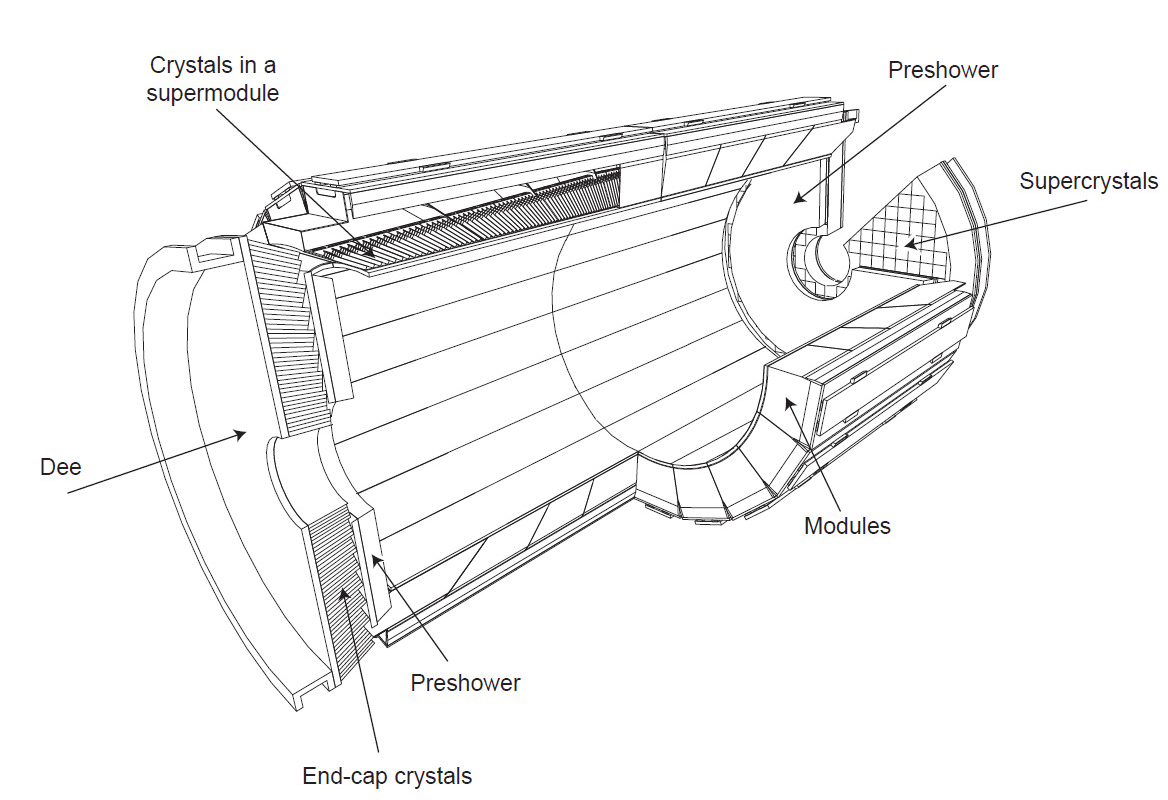
\includegraphics[width=0.8\textwidth]{figures/ecal}
  \caption[Layout of the CMS electromagnetic calorimeter]{Layout of the CMS electromagnetic calorimeter~\cite{1748-0221-3-08-S08004}.}
  \label{fig:ecal}
\end{figure}
Surrounding the tracker, the ECAL (shown in~\cref{fig:ecal}) is composed of
transparent lead-tungstate scintillator crystals. Lead-tungstate was chosen
because of its radiation hardness, fast light output (\SI{80}{\percent} in
\SI{25}{\nano\second}), short radiation length (the mean distance an incoming
electron traverses before losing all but $1/\Pe$ of its energy) of
\SI{0.89}{\centi\meter}, and a small Moli\`er radius (the radius of a cylinder
containing \SI{90}{\percent} of the shower energy) of \SI{2.2}{\centi\meter}. A
short radiation length and small Moli\`er radius is desirable in order to fully
absorb incoming particles with a compact design. The electromagnetic shower
induced in the crystals causes the energized scintillator atoms to emit light in
proportion to the size of the shower. This scintillation light is collected by
avalanche photodiodes in the barrel and photomultiplier devices called vacuum
phototriodes in the endcaps. There are \num{61000} crystals in the ECAL barrel
region, which covers $|\eta| < 1.479$, and \num{7324} crystals in each of the
ECAL endcaps, covering $1.479 < |\eta| < 3$. The crystals vary
between~\SIrange{22}{23}{\centi\meter} in length.

A finer-grained detector, the ECAL preshower (ES), is placed in front of each
endcap. It has a total thickness of about \SI{20}{\centi\meter} and uses a
sampling design consisting of two layers of lead radiators to induce showers,
interleaved with two layers of silicon strip sensors to measure the deposited
energy. The intended function of the ES was to help distinguish $\pi^0
\rightarrow \gamma\gamma$ decays from single high-energy prompt photons.
Unfortunately, the large number of neutral pions produced through hadronic
interactions with the tracker material in practice degrades the ES capabilities
and thus the energy deposits in the ES are simply added to corresponding
deposits in the ECAL.

Over time, radiation induces lattice damage in the lead tungstate crystals and
reduces their transparency. Consequently, a calibration system is necessary.
This system uses the LHC abort gaps to measure the baseline electronic noise
(\textit{pedestal}) levels and fire laser or LED pulses into the crystals to
measure their transparency at regular intervals during data collection (on the
order of once per hour).

\subsubsection{Hadronic calorimeter}
The HCAL is a sampling calorimeter composed of interleaved layers of brass
absorber and tiles of plastic scintillator material. Brass is an ideal material
for this purpose because it is non-magnetic and has a relatively short
interaction length (\SI{16.4}{\centi\meter}), which is the average distance a
particle will travel before interacting with the absorber. The HCAL surrounds
the ECAL, and extends radially between \SIrange{1.77}{2.95}{\meter} from the
beamline, providing a minimum of six interaction lengths for hadrons passing
through it.

Incident hadrons cause showers of hadrons and leptons in the brass, which causes
light to be produced in the scintillating layers in proportion to the amount of
energy deposited. The light from the tiles is collected by wavelength-shifting
fibers that are grouped into readout towers before being transmitted to hybrid
photodiodes for amplification and readout.

The HCAL barrel (HB) region covers $|\eta| < 1.3$, and there are two HCAL end
caps (EC), with each covering $1.3 < |\eta| < 3$. The EC and HB sections do not
fully absorb all hadronic showers; any components passing beyond the HCAL are
referred to as \textit{hadronic punchthrough}. To measure shower energy
deposited outside the HB, there is an extra layer of scintillator tiles located
outside the solenoid, concentric to the HB, called the HCAL outer, or tail
catcher. This outer layer uses the solenoid coil itself as an absorber. At
either end of CMS, there are additional sections called the HCAL forward (HF)
that covers $4.5 < \abs{\eta} < 5.2$ and absorbs particles emerging from the IP
at shallow angles. The HF absorbs the majority of the energy from the collision
and so is made of steel absorber plates interleaved with layers of quartz
fibers; interactions in the absorber produce showers of particles that pass
through the quartz fibers, generating flashes of Cerenkov light.

\subsection{Muon subsystem}
\begin{figure}[htb]
  % \centering
  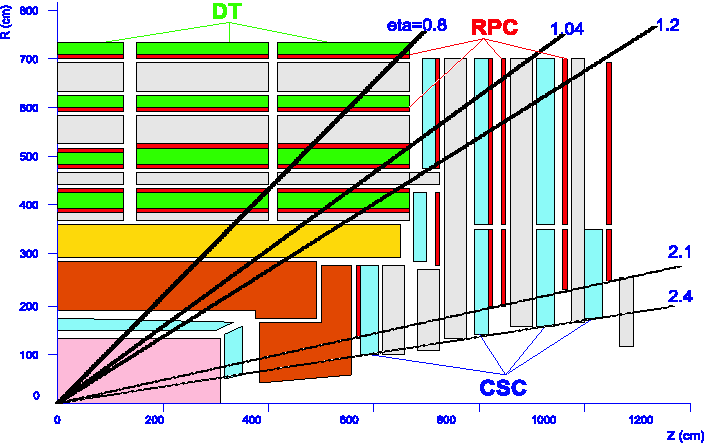
\includegraphics[width=\textwidth]{figures/muon_quadrant}
  \caption[Cross section of one quadrant of the CMS muon system]{An $R-Z$ cross section of one quadrant of the CMS muon system~\cite{cms-tdr-1}.}
  \label{fig:muonquadrant}
\end{figure}
Muons lose less energy due to bremsstrahlung than electrons because of their
higher mass and do not interact via the strong force. Consequently the CMS muon
subsystem~\cite{muonTDR} is the outermost detector since muons are the only
charged particle that makes it that far. Since the mass of the particle is
known, it is only necessary to measure its charge and momentum.

The muon tracker (MT) subsystem consists of a cylindrical barrel region and two
endcaps. The barrel is divided along the beam axis into five separate wheels
with four concentric layers, alternating with layers of the return yoke.
Throughout Run 1, the endcaps had three disks (\textit{stations}) each; during
LS1 a fourth disk was installed~\cite{Guiducci:1966038}.

Because it is so far from the IP, the MT must cover a much greater area than the
inner trackers to be hermetic. Consequently it must be less expensive per unit
area to be practical; however, it does not require as high a resolution as the
inner detectors. Gas ionization chambers of three types were selected.

Drift tubes (DTs) are used in the barrel region because it has lower muon rates.
There are four layers of stations covering $\abs{\eta} < 1.2$. The DTs consist
of $\SI{13}{\mm} \times \SI{42}{\mm} \times \SI{2.4}{\meter}$ cells filled with
a mixture of carbon dioxide and argon gas. An anode wire held at a positive
potential of \SI{3.6}{\kilo\volt} runs the length of the tube, while electrode
strips on the \SI{42}{\mm} walls are held at \SI{1.8}{\kilo\volt} and on the
\SI{13}{\mm} walls are held at \SI{-1.2}{\kilo\volt}. A muon passing through the
tube ionizes the gas, producing free electrons and positively charged ions that
drift to the wire or strips, creating a signal that is amplified and measured.
Groups of four cells are stacked, staggered by half a cell to eliminate dead
spots, to form a superlayer (SL). The DTs are arranged in four concentric
cylinders around the beam axis, called stations, which alternate with layers of
the steel plates that form the magnet return yoke. The three inner stations have
three SLs each; two have wires running parallel to the beamline in order to
measure $r-\phi$ and one has wires perpendicular to the beamline in order to
measure $\eta$. The outer station has two SLs with wires that are parallel to
the beam and only measure $r-\phi$.

Cathode strip chambers (CSCs) with higher resolution than the drift tubes are
used in the endcaps, where the magnetic field is nonuniform and the muon rates
are higher. Each endcap has four disks of CSCs covering $1.2 < \abs{\eta} <
2.4$. As with the barrel, the disks alternate with steel plates of the return
yoke. Each CSC is trapezoidal in shape with seven layers of cathode panels that
have strips at constant $\phi$ intervals pointing radially out from the beam.
These are interleaved with six panels of anode wires, oriented roughly
perpendicularly to the cathode strips, to measure the radial position of the
hit. Between the panels is a mixture of carbon dioxide, argon, and carbon
tetrafluoride. CSCs use a mechanism similar to the DTs. An electrostatic
potential is maintained between the anodes and cathodes; incoming muons ionize
gas molecules, producing ions that drift towards the wire or strips, creating a
small current pulse that is amplified and recorded.

Resistive plate chambers (RPCs) are gaseous parallel-plate detectors. The
mechanism of operation is similar to the CSCs, except that there is a very
narrow gap of \SI{2}{\milli\meter} between the charged plates. This gap means
they have a lower spatial resolution, but a very fast response time of only one
nanosecond. Because the CSCs and DTs alone are not fast enough to unambiguously
associate muons with a specific bunch crossing, RPCs are used throughout the
system, covering the entire range of pseudorapidity.

The spatial resolution achieved per chamber is \SIrange{80}{120}{\micro\meter}
in the DTs, \SIrange{40}{150}{\micro\meter} in the CSCs, and
\SIrange{8}{12}{\milli\meter} in the RPCs. The efficiency for reconstructing
hits and track segments in the muon system is in the range
\SIrange{95}{98}{\percent}~\cite{Chatrchyan:2013sba}.

\subsection{Trigger and data acquisition}
Each crossing between two bunches of protons at the IP in which protons collide
is called an \textit{event}. During Run 1, the LHC normally provided $pp$
collisions with a bunch spacing of \SI{50}{\nano\second}. In Run 2, the bunch
spacing was reduced to \SI{25}{\nano\second}. This corresponds to a peak (in
other words, excluding abort gaps) crossing frequency of \SI{20}{\mega\Hz} and
\SI{40}{\mega\Hz} for Run 1 and Run 2, respectively. The raw information read
out by the detector for each event is $\mathcal{O}(\SI{500}{kB})$, meaning that
CMS produces tens of terabytes of data per second, far exceeding the pace at
which the data can be recorded. This rate necessitates a \textit{trigger} system
that quickly selects the most interesting events for storage. Discarded data
cannot be recovered, so a properly functioning trigger system is critical to the
success of the experiment. Periods during which events are not recorded because
systems are busy processing existing data are referred to as \emph{dead time}
and should be minimized. The event rate is reduced in two stages: first, a
faster, hardware-based Level 1 (L1) trigger reduces the event rate to
\SIrange{80}{100}{\kilo\hertz}. Next, a slower, software-based High Level
Trigger (HLT) further reduces the event rate to approximately
\SI{1}{\kilo\hertz}.

The time between the collision and when the L1 delivers a final decision is
referred to as the \emph{latency}. During this time, all of the data from the
detector are buffered in a pipeline before being either discarded or forwarded
on to the HLT. The L1 latency is \SI{4}{\micro\sec}, which coincides with the
length of the LHC abort gap, making it possible to operate with zero dead time.
This goal is accomplished with fast electronics (field programmable gate arrays)
that construct local \emph{trigger primitives} from the raw output of the
calorimeters and muon systems (track reconstruction is too computationally
expensive to complete on the L1 timescale). The calorimeter output channels are
grouped into trigger towers. Trigger primitive generators calculate $E_T$ sums
for each tower and send them to the Regional Calorimeter Trigger, which combines
these values with quality information about the shower pattern to identify
candidate electrons and photons, along with $E_T$ sums for groups of $4 \times
4$ towers. These quantities are then passed to the Global Calorimeter Trigger
(GCT), which calculates the sum $E_T$, \pTmiss and the scalar sum of transverse
energy $H_T$. Track segments and hit patterns from the DT and CSC local triggers
are sent in parallel to their respective track finders, which sort the trigger
primitives by \pT and quality. Information is shared between the two track
finders so that overlapping track segments can be linked. The RPCs assemble muon
candidates from regional hit patterns and, because they are much faster than the
CSCs and DTs, provide unambiguous bunch crossing identification. The best
candidates from all three systems are passed on to the Global Muon Trigger
(GMT), which combines the information for improved momentum resolution and
efficiency.

The highest-quality objects (i.e., electrons/photons, muons, jets, or \Ptau
leptons) from the GCT and GMT are forwarded to the Global Trigger (GT). A
\textit{path} is a set of algorithms and requirements on objects in an event. L1
paths have simple criteria; for example, the event must contain at least one
muon exceeding a given threshold, or the event must contain combinations of
several objects. A trigger menu with a maximum of 128 different paths could be
specified during Run 1. During LS1, the L1 trigger was
upgraded~\cite{Tapper:1556311}, which added several L1 improvements, including
adding fast pileup subtraction and expanded the menu size to a maximum of 256
paths.

If an event satisfies the criteria of any path in the L1 menu, the GT sends an
L1 Accept signal to the Timing, Trigger, and Control (TTC) system which controls
readout of the subdetector frontend buffers to the front-end drivers (FEDs). FED
fragments are subsequently merged by the Event Builder and passed to the HLT.
The HLT is a version of the sophisticated event reconstruction software used in
offline analysis and achieves similar quality reconstruction. The HLT had a per
event time budget of \SI{175}{\sec} during 2012. This longer timescale is made
possible by a computer cluster with \num{13000} cores which can process multiple
events simultaneously. The HLT menu is composed of more than \num{400} paths.
HLT paths are more complex than at L1, consisting of a sequence of
reconstruction and filtering steps. Products are filtered as algorithms are run.
In this way, selections relying on calorimeter and muon system data, which are
run first, reduce the number of events over which the computationally expensive
tracker reconstruction is performed.

More details on the trigger system can be found
in~\cite{1748-0221-12-01-P01020}.

